% Options for packages loaded elsewhere
\PassOptionsToPackage{unicode}{hyperref}
\PassOptionsToPackage{hyphens}{url}
\PassOptionsToPackage{dvipsnames,svgnames*,x11names*}{xcolor}
%
\documentclass[
  11pt,
]{article}
\usepackage{lmodern}
\usepackage{amssymb,amsmath}
\usepackage{ifxetex,ifluatex}
\ifnum 0\ifxetex 1\fi\ifluatex 1\fi=0 % if pdftex
  \usepackage[T1]{fontenc}
  \usepackage[utf8]{inputenc}
  \usepackage{textcomp} % provide euro and other symbols
\else % if luatex or xetex
  \usepackage{unicode-math}
  \defaultfontfeatures{Scale=MatchLowercase}
  \defaultfontfeatures[\rmfamily]{Ligatures=TeX,Scale=1}
\fi
% Use upquote if available, for straight quotes in verbatim environments
\IfFileExists{upquote.sty}{\usepackage{upquote}}{}
\IfFileExists{microtype.sty}{% use microtype if available
  \usepackage[]{microtype}
  \UseMicrotypeSet[protrusion]{basicmath} % disable protrusion for tt fonts
}{}
\makeatletter
\@ifundefined{KOMAClassName}{% if non-KOMA class
  \IfFileExists{parskip.sty}{%
    \usepackage{parskip}
  }{% else
    \setlength{\parindent}{0pt}
    \setlength{\parskip}{6pt plus 2pt minus 1pt}}
}{% if KOMA class
  \KOMAoptions{parskip=half}}
\makeatother
\usepackage{xcolor}
\IfFileExists{xurl.sty}{\usepackage{xurl}}{} % add URL line breaks if available
\IfFileExists{bookmark.sty}{\usepackage{bookmark}}{\usepackage{hyperref}}
\hypersetup{
  pdftitle={Tutorial-4},
  pdfauthor={Eyayaw Beze},
  colorlinks=true,
  linkcolor=blue,
  filecolor=Maroon,
  citecolor=Blue,
  urlcolor=Blue,
  pdfcreator={LaTeX via pandoc}}
\urlstyle{same} % disable monospaced font for URLs
\usepackage[margin=1in]{geometry}
\usepackage{graphicx}
\makeatletter
\def\maxwidth{\ifdim\Gin@nat@width>\linewidth\linewidth\else\Gin@nat@width\fi}
\def\maxheight{\ifdim\Gin@nat@height>\textheight\textheight\else\Gin@nat@height\fi}
\makeatother
% Scale images if necessary, so that they will not overflow the page
% margins by default, and it is still possible to overwrite the defaults
% using explicit options in \includegraphics[width, height, ...]{}
\setkeys{Gin}{width=\maxwidth,height=\maxheight,keepaspectratio}
% Set default figure placement to htbp
\makeatletter
\def\fps@figure{htbp}
\makeatother
\setlength{\emergencystretch}{3em} % prevent overfull lines
\providecommand{\tightlist}{%
  \setlength{\itemsep}{0pt}\setlength{\parskip}{0pt}}
\setcounter{secnumdepth}{-\maxdimen} % remove section numbering
\usepackage{multirow}
\usepackage{booktabs}
\usepackage{float}
\floatplacement{figure}{H}
\newlength{\cslhangindent}
\setlength{\cslhangindent}{1.5em}
\newenvironment{cslreferences}%
  {\setlength{\parindent}{0pt}%
  \everypar{\setlength{\hangindent}{\cslhangindent}}\ignorespaces}%
  {\par}

\title{Tutorial-4}
\author{Eyayaw Beze}
\date{June 21, 2020}

\begin{document}
\maketitle

\hypertarget{exercise-1-did---paper-discussion}{%
\section{Exercise 1: DiD - paper
discussion}\label{exercise-1-did---paper-discussion}}

\hypertarget{research-question}{%
\subsection*{Research question}\label{research-question}}
\addcontentsline{toc}{subsection}{Research question}

Are supply-side drug control efforts effective? The study attempted to
answer this question by focusing on the state and federal restrictions
on OTC medicines containing methamphetamine precursors in the US.

\hypertarget{contribution}{%
\subsection*{Contribution}\label{contribution}}
\addcontentsline{toc}{subsection}{Contribution}

The study indicated that there is no consensus in the literature
regarding the effectiveness of enforcement efforts in reducing drug use.
As a result, the paper contributes to the existing literature by
providing concrete empirical evidence on the effectiveness of
enforcement efforts by using rich administrative records and the
staggered implementation of state laws targeting over-the-counter
medicines that can be used to produce methamphetamine.

More precisely, the authors indicated that their paper contributes to
the literature by providing more credible estimates of the effect of
analyzing the success of a smaller, but more typical enforcement effort.

\hypertarget{aim-of-the-analyzed-policy}{%
\subsection*{Aim of the analyzed
policy}\label{aim-of-the-analyzed-policy}}
\addcontentsline{toc}{subsection}{Aim of the analyzed policy}

The legislation's aim is preventing the diversion of ephedrine or
pseudoephedrine (precursors of methamphetamine) to methamphetamine
production and hence reduce its availability.

\hypertarget{methodology}{%
\subsection*{Methodology}\label{methodology}}
\addcontentsline{toc}{subsection}{Methodology}

\begin{itemize}
\tightlist
\item
  The authors examine the effect of the laws using a
  difference-in-difference model where the treatment is at the state
  level, with controls for state and month/year fixed effects and
  state-specific time trends.
\item
  Additionally, event studies are used to support the validity of the
  main conclusions of the paper and to provide insight about the dynamic
  effects of the OTC restrictions.
\end{itemize}

\hypertarget{identifying-variation}{%
\subsection*{Identifying variation}\label{identifying-variation}}
\addcontentsline{toc}{subsection}{Identifying variation}

Geographic (states) as well as temporal variation in the implementation
of the regulation: the paper exploited the variation in the timing of
states' implementation of OTC regulations.

\hypertarget{key-identifying-assumption}{%
\subsection*{Key identifying
assumption}\label{key-identifying-assumption}}
\addcontentsline{toc}{subsection}{Key identifying assumption}

As noted above, there is variation in the timing of state OTC
regulations. The paper aimed at separately identifying the effects of
the regulations from common changes in outcomes across all states. Thus,
the identification assumption is once we control for state fixed and
year/month effects (linear or nonlinear), there are no unmeasured
state-level non-linear trends that are correlated with methamphetamine
production and consumption and the introduction of the OTC restrictions.

\hypertarget{data}{%
\subsection*{Data}\label{data}}
\addcontentsline{toc}{subsection}{Data}

The study compiled data from multiple sources.

\begin{itemize}
\tightlist
\item
  Number of methamphetamine labs, from The National Clandestine Lab
  Seizure System (NCLSS),\\
\item
  The price and purity of methamphetamine, from Drug Enforcement
  Agency's System to Retrieve Information (STRIDE),\\
\item
  Positive drug tests for amphetamine among workers and hospital
  inpatients, from Quest Diagnostics and the Health Care Utilization
  Project (HCUP), and\\
\item
  Drug-related arrests, from Uniform Crime Reports (UCR)
\end{itemize}

\hypertarget{results-findings}{%
\subsection*{Results / findings}\label{results-findings}}
\addcontentsline{toc}{subsection}{Results / findings}

\begin{itemize}
\item
  The paper estimates that OTC restrictions reduced total
  methamphetamine production capacity within a state by 26\%.
\item
  The OTC restrictions significantly decreased within-state
  methamphetamine production---the estimate that the laws caused a
  reduction in the number of methamphetamine laboratories being 36\%.
  The reduction in the number of labs was largest among the laboratories
  with the smallest production capacities, but it was relatively small
  in the number of larger laboratories.
\item
  According to the paper's estimate, there is about 25\% decline in
  overall domestic production of methamphetamine.
\item
  However, the study found no evidence about the impact of the OTC
  restrictions on the purity, price and consumption of methamphetamine,
  and drug related arrests.
\item
  Evidence for the spatial spillover effect of the intervention on
  border/neighboring counties/states.
\end{itemize}

\hypertarget{interpretation-of-the-results-implications-policy-relevance}{%
\subsection*{Interpretation of the results / implications / policy
relevance}\label{interpretation-of-the-results-implications-policy-relevance}}
\addcontentsline{toc}{subsection}{Interpretation of the results /
implications / policy relevance}

I summarize the implications of the findings of the paper as follows.

\begin{itemize}
\item
  The OTC laws successfully disrupted local methamphetamine production;
  the number of meth-labs in the state has declined significantly (by
  about 40\%). Reductions apply to laboratories of all sizes, but the
  largest and most significant reductions were among the smaller
  laboratories.
\item
  Despite the large reduction in the production of methamphetamine
  within a state, the study finds no evidence of reductions in
  methamphetamine purity, consumption, or arrests. This is worrisome as
  the goal of the legislation was to cut the supply of methamphetamine
  so that people's drug consumption are curtailed or at least
  controlled.
\item
  Highlighting the possible policy implications of the paper requires
  answering the question why the legislation's effectiveness (in
  significantly reducing methamphetamine supply) did not translate into
  reductions in drug consumption (in terms of price as well as quality)
  and drug related arrests. It would require providing broader insight
  about the interplay between the overall drug supply and demand markets
  in the US and neighboring countries, especially in Mexico. Because,
  for example having a bulk production of close substitutes to
  methamphetamine in the US and the possibility of import from Mexico
  and other Latin American countries would obscure the effects of the
  regulations. In fact, the study finds evidence that methamphetamine
  producers in border counties responded to the OTC laws by purchasing
  precursors in neighboring states that did not have a law in place.
  This reduced the effectiveness of the laws and as purchasing and
  transporting a legal product involves low if not no risk.
\end{itemize}

\hypertarget{limitations-of-the-paper}{%
\subsection*{Limitations of the paper}\label{limitations-of-the-paper}}
\addcontentsline{toc}{subsection}{Limitations of the paper}

One clear limitation of the paper is the data. While acknowledging the
fact that the ideal data for measuring the effect of the laws on
methamphetamine production would be a census of labs for each state
spanning before and after the laws went into effect, the study relied on
the number of labs discovered by law enforcement agents as a measure for
the outcome variable(s). However, the number of labs discovered each
month is just an unknown fraction of the total number of labs in
operation that month. Thus, the outcome variable is clearly understated.

Moreover, the findings are based on the assumption that the probability
of a lab being seized remains constant even after the introduction of
the law. But following the regulation enactment, it is likely that the
detection probability would change afterwards. For example, the
investigation efforts of law enforcement agents may go down, reports
from the public may increase as the public has now law protection due to
the new regulations for exposing offenders. These possibilities are not
considered in the paper.

The results on drug use might suffer from selection bias in the
measurement of methamphetamine consumption as it is likely that only
patients and workers with a previous record of drug use are subject to
methamphetamine consumption tests.

In terms of the policy objective, the general problem of drug abuse and
violence might remain unalleviated if the regulation restrictions do not
also apply to the substitutes to methamphetamine and other types of
drugs. Special attention should also be accorded to producers that are
more experienced and have widely established production and distribution
networks since the detection likelihood of such firms is low. Moreover,
the policy implications of the paper cannot be extrapolated to all drugs
that are available for consumption for in the US since some drugs are
mainly imported from neighboring countries. In addition, coordination
among states and also with the federal government could have made the
policy more effective.

\hypertarget{exercise-2-did---practical-application}{%
\section{Exercise 2: DiD - practical
application}\label{exercise-2-did---practical-application}}

\begin{enumerate}
\def\labelenumi{(\alph{enumi})}
\tightlist
\item
  \textbf{Reproduce Figure (2) of (Dobkin, Nicosia, and Weinberg
  \protect\hyperlink{ref-DOBKIN201448}{2014})}
\end{enumerate}

The two points mentioned in the paper corresponding to this figure can
also be seen in this plot (see Figure (\ref{fig-1})). First, for each
group, there was a decrease in the average number of labs discovered
beginning in early 2004. Second, by 2007 the average number of labs
discovered in a state was less than half of what it was before 2004 for
each of the three groups of labs. However, these declines in the number
of labs from 2004 to 2007 were not solely due to the OTC regulations, as
the declines began before states enacted the sales restrictions. This
fact is further supported by Figure (\ref{fig-2}).

\begin{figure}[H]
 \centering
 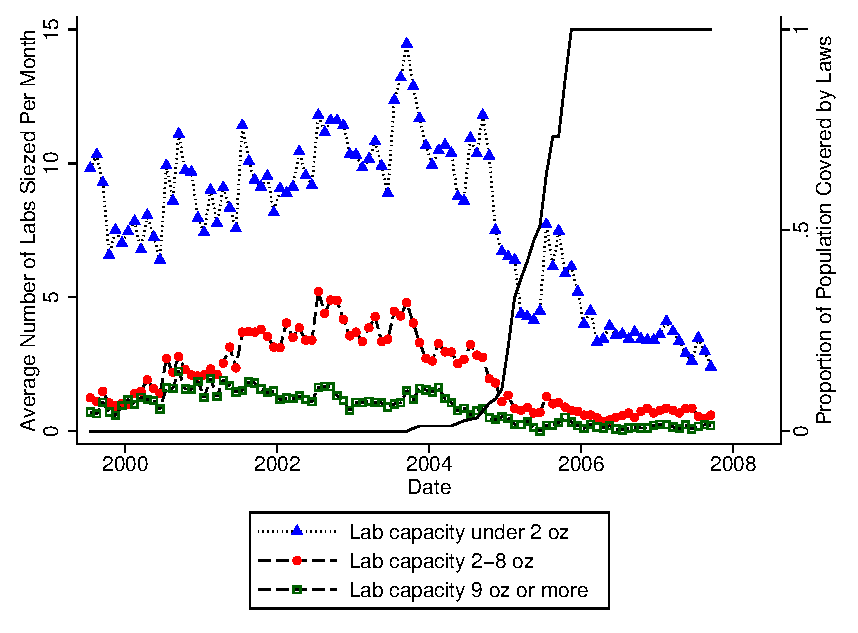
\includegraphics{number_of_labs_siezed-timeseries.eps}
 \caption{Methamphetamine labs discovered or seized by capacity. \\ The
figure contains the average number of labs discovered in a state by
month.}
\label{fig-1}
\end{figure}

\begin{enumerate}
\def\labelenumi{(\alph{enumi})}
\setcounter{enumi}{1}
\tightlist
\item
  \textbf{Make a graph that shows the average number of the three
  different types of labs discovered in event time. Center the figure at
  time 0 (when the law went into effect in the state).}
\end{enumerate}

The number of labs seized (in each group) started declining before the
states implemented the regulations, roughly a year (12 months) before
the law came into effect, as can be seen in Figure (\ref{fig-2}).

\begin{figure}[hbt!]
 \centering
 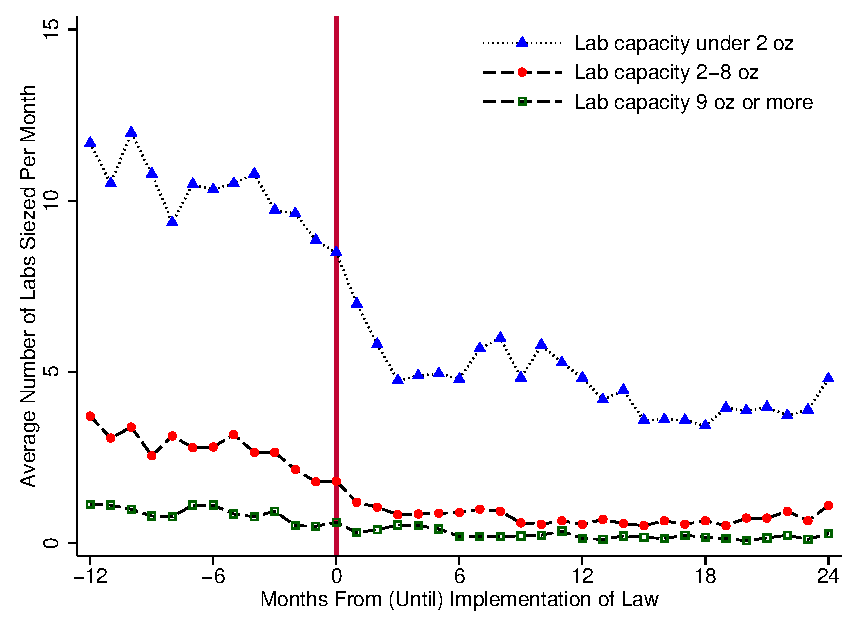
\includegraphics{month_from_until_otc-vs-lab_size.eps}
 \caption{Methamphetamine labs discovered or seized by capacity in event time.\\ The figure contains the average number of labs discovered in a state by month.}
\label{fig-2}
\end{figure}

\begin{enumerate}
\def\labelenumi{(\alph{enumi})}
\setcounter{enumi}{2}
\tightlist
\item
  \textbf{Estimate a standard FE model to determine the effect of the
  law on the number of discovered labs of the three different sizes.
  Equation (\ref{eq:1}) of (Dobkin, Nicosia, and Weinberg
  \protect\hyperlink{ref-DOBKIN201448}{2014}) serves as your reference
  point. Be sure to code the \(OTC_{st}\) indicator as defined in the
  paper. Use the appropriate standard errors and justify your choice. Do
  your coefficients coincide with what you see in your graphs and with
  the regression estimates of the paper?}
\end{enumerate}

Following the paper's definition of the variable of interest OTC
regulation, I coded \(OTC_{st}\) as follows.

\[OTC_{st} = \begin{cases} 
      0 & event.date_{month} < any.law_{month} \\
      \frac{end.of.month-event.date-1}{end.of.month} & event.date_{month} = any.law_{month} \\
      1 & event.date_{month} > any.law_{month}
   \end{cases}\]

\begin{table}[!htbp]\centering
\def\sym#1{\ifmmode^{#1}\else\(^{#1}\)\fi}
\caption{Impact of OTC regulations on methamphetamine lab seizures.}
\begin{tabular}{l*{8}{c}}
\midrule\midrule
\multicolumn{1}{l}{ } & \multicolumn{4}{l}{Number of Labs Seized } & \multicolumn{4}{l}{ Lab capacity under 2 oz \label{fe-results}}\\ \cmidrule(l{3pt}r{3pt}){2-5} \cmidrule(l{3pt}r{3pt}){6-9}
 &\multicolumn{1}{l}{(1)}&\multicolumn{1}{l}{(2)}&\multicolumn{1}{l}{(3)}&\multicolumn{1}{l}{(4)}&\multicolumn{1}{l}{(1)}&\multicolumn{1}{l}{(2)}&\multicolumn{1}{l}{(3)}&\multicolumn{1}{l}{(4)}\\
\midrule
OTC\_Restriction& -6.593\sym{**} & -6.601\sym{**} & -4.830\sym{**} & -5.523\sym{***}& -4.075\sym{**} & -4.077\sym{**} & -2.893\sym{**} & -3.424\sym{***}\\
\midrule
Mean & 10.90 & 10.90 & 10.90 & 10.90 & 7.834 & 7.834 & 7.834 & 7.834 \\
Observations& 4937 & 4937 & 4937 & 4937 & 4937 & 4937 & 4937 & 4937 \\
States & 50 & 50 & 50 & 50 & 50 & 50 & 50 & 50 \\
\midrule\midrule
\vspace{0.5cm}\\
\multicolumn{1}{l}{ } & \multicolumn{4}{l}{Lab capacity 2-8 oz } & \multicolumn{4}{l}{ Lab capacity 9 oz or more }\\ \cmidrule(l{3pt}r{3pt}){2-5} \cmidrule(l{3pt}r{3pt}){6-9}
 &\multicolumn{1}{l}{(1)}&\multicolumn{1}{l}{(2)}&\multicolumn{1}{l}{(3)}&\multicolumn{1}{l}{(4)}&\multicolumn{1}{l}{(1)}&\multicolumn{1}{l}{(2)}&\multicolumn{1}{l}{(3)}&\multicolumn{1}{l}{(4)}\\
\midrule
OTC\_Restriction& -2.251\sym{***}& -2.258\sym{***}& -1.752\sym{***}& -1.940\sym{***}& -0.266 & -0.266 & -0.185 & -0.158 \\
\midrule
Mean & 2.177 & 2.177 & 2.177 & 2.177 & 0.890 & 0.890 & 0.890 & 0.890 \\
Observations& 4937 & 4937 & 4937 & 4937 & 4937 & 4937 & 4937 & 4937 \\
States & 50 & 50 & 50 & 50 & 50 & 50 & 50 & 50 \\
\midrule\midrule
\multicolumn{9}{l}{\footnotesize Notes: All regressions include state fixed effects and year/month fixed effects.}\\
\multicolumn{9}{l}{\footnotesize The dependent variable in the regressions is count of labs seized or discovered in a month in a particular state.}\\
\multicolumn{9}{l}{\footnotesize \sym{*} \(p<0.05\), \sym{**} \(p<0.01\), \sym{***} \(p<0.001\)}\\
\end{tabular}
\end{table}

I estimate the 4 models of the paper starting from model (\ref{eq:1})
and then by progressively adding state-specific linear time trend in
(\ref{eq:2}), quadratic state-specific time trends in (\ref{eq:3}), and
in the last one (\ref{eq:4}) adding two covariates, the unemployment
rate and the number of households receiving food stamps. The results of
the estimations are reported in Table (\ref{fe-results}). And, my
coefficients look to roughly match the estimates reported in Table 1 of
(Dobkin, Nicosia, and Weinberg
\protect\hyperlink{ref-DOBKIN201448}{2014}). They slight differences are
due to the fact that we include the whole time period of the sample and
the data for the state of Florida was missing.

The results of each of the models coincide with what we see on the
plots. There is a statistically significant strong negative effect of
the law on the number of labs seized for each category of labs,
specially the effects are more pronounced in smaller labs. The magnitude
of the slope coefficients increase as we add more and more controls to
the baseline model (\ref{eq:1}) (exception being large labs). None of
the coefficients are statistically significant when the outcome variable
is \texttt{Lab\ capacity\ 9\ oz\ or\ more}.

\begin{align}
& Y_{s t}=\beta O T C_{s t} + \alpha_{s} + \gamma_{t} + \epsilon_{s t}
\label{eq:1}\\
& Y_{s t}=\beta O T C_{s t} + \alpha_{s} + \gamma_{t} + \delta_{s} \cdot t + \epsilon_{s t}\label{eq:2} \\
& Y_{s t}=\beta O T C_{s t} + \alpha_{s} + \gamma_{t} + \delta_{s} \cdot t + \Delta_{s} \cdot t^2 + \epsilon_{s t}\label{eq:3} \\
& Y_{s t}=\beta O T C_{s t} + \alpha_{s} + \gamma_{t} + \delta_{s} \cdot t + \Delta_{s} \cdot t^2 + \theta_1FOOD_{st} + \theta_{2} UNEMP_{st} + \epsilon_{s t} \label{eq:4}
\end{align}

\textbf{\large Comment on Cluster Standard Errors}

Abadie et al. (\protect\hyperlink{ref-Abadie2017}{2017}) argue that
clustering is in essence a design problem, either a sampling design or
an experimental design issue. Since the states are not selected
randomly, and since there are not clusters in the population of interest
(the country United States) beyond the 50 (plus 1) clusters that are
seen in the sample, the second design issue suitably applies to this
paper. Clustering due to an experimental design is if the treatment is
correlated within the clusters. I think that the treatment (OTC
regulation) is correlated within clusters, i.e., states.

However, one may ask why do we care about cluster standard errors when
we use fixed effects? Including fixed effects in the regression function
to account for the clusters, thinking that the fixed effects completely
eliminate the within-cluster correlation of the residuals, does not rule
out the need for cluster standard errors adjustments. In case of fixed
effects, cluster standard errors should be used if there is
heterogeneity in the treatment effects.

States implemented the OTC regulations at different times, and this is
in fact the motivation for the study. The timing of the treatment then
depends which state we are referring to. Thus, I think unobserved
components in outcomes (residuals) (and also observed ones-regressors)
for individual units (lab seizures) within clusters are correlated.

Therefore, the existence of variation in the timing of state OTC
regulations necessitates the use for cluster standard errors. Hence,
there should be clusters at the state level---the highest level of
aggregation in the sample.

\begin{enumerate}
\def\labelenumi{(\alph{enumi})}
\setcounter{enumi}{3}
\tightlist
\item
  \textbf{Under what assumptions does equation (\ref{eq:1}) of the paper
  reveal consistent estimates? Do you think that these assumptions are
  met?}
\end{enumerate}

\begin{itemize}
\item
  Unbiasedness of the DiD estimator (Assumption DID.2): which requires
  that the policy change not be systematically related to other factors
  that affect the outcome variables (lab seizures) (and are hidden in
  the error term). State and time invariant effects are not correlated
  with the error term. I think it's hardly true that this assumption is
  met, because the model does not account for state specific (time
  varying such as state unemployment rate) covariates.
\item
  Consistency of the DiD estimator: which requires that there are no
  state specific trends that are correlated with the treatment---OTC
  restriction. Time fixed effects were included to account for aggregate
  common changes over time. \textbf{DiD common trend assumption}
  (Assumption DID.4 (Common Trend - CT)).
\item
  No pre-trend (Assumption DID.3 (No Effect Prior to Treatment - NEPT)):
  This assumption has been tested in the paper through event study
  analysis. The paper indicated that event study analysis not only
  allows to examine any ``pre-trend'' that would raise concerns about
  the identification but also to determine exactly when the regulations
  had an impact and how persistent it might be.
\item
  Broadly, assumptions DiD1-DiD5
\end{itemize}

\begin{enumerate}
\def\labelenumi{(\alph{enumi})}
\setcounter{enumi}{4}
\tightlist
\item
  \textbf{What does equation (\ref{eq:1}) assume about the temporal
  evolution of the treatment effect? How does the regression equation
  (\ref{eq:2}) of the paper improve on this?}
\end{enumerate}

Equation (\ref{eq:1}) (implicitly) assumes the treatment effect to be
constant over time; \(\beta\) (the effect of the treatment) do not vary
across states and time. In contrast, in equation (\ref{eq:2}) the
treatment effect is allowed to vary over time, but still no variation
across states. We can say this is an improvement over the baseline
model, because equation (\ref{eq:2}) captures the temporary evolution of
the treatment.

\begin{enumerate}
\def\labelenumi{(\alph{enumi})}
\setcounter{enumi}{5}
\tightlist
\item
  \textbf{Similar to equation (\ref{eq:2}) of the paper, run a
  regression of the number of labs discovered on state FE, time dummies
  and event time dummies. Plot the estimates of the event time dummies
  and their confidence intervals. Interpret the figure and compare it
  with your previous findings. Did the laws reduce the number of labs?
  Does the effect look persistent?}
\end{enumerate}

We estimate the following model:

\begin{equation}
Y_{s t}=\sum_{j=-12}^{24} \pi_{j} 1\left(\tau_{s t}=j\right)+\alpha_{s}+\gamma_{t}+\delta_{s} * t+\epsilon_{s t}
\end{equation}

The estimated \(\pi_{j}\) coefficients with their 95 percent confidence
intervals are plotted below against event time dummies for
\(j \in [-12, 24]\) for each category of lab sizes.

In terms of the effects of the treatment, what the confidence interval
plots show is consistent with the previous findings (cf.~Table
\ref{fe-results}). The reductions in the number of small labs are
substantial due to the regulation. The effect on large labs is not
significant since the 95 percent confidence intervals of the \(\pi_j\)
coefficients include zero (see \ref{ci-cap9})---consistent with the
findings in the above regression models (see (c)). Yes, the effect looks
persistent to me.

\begin{figure}[!hbtp]
 \centering
 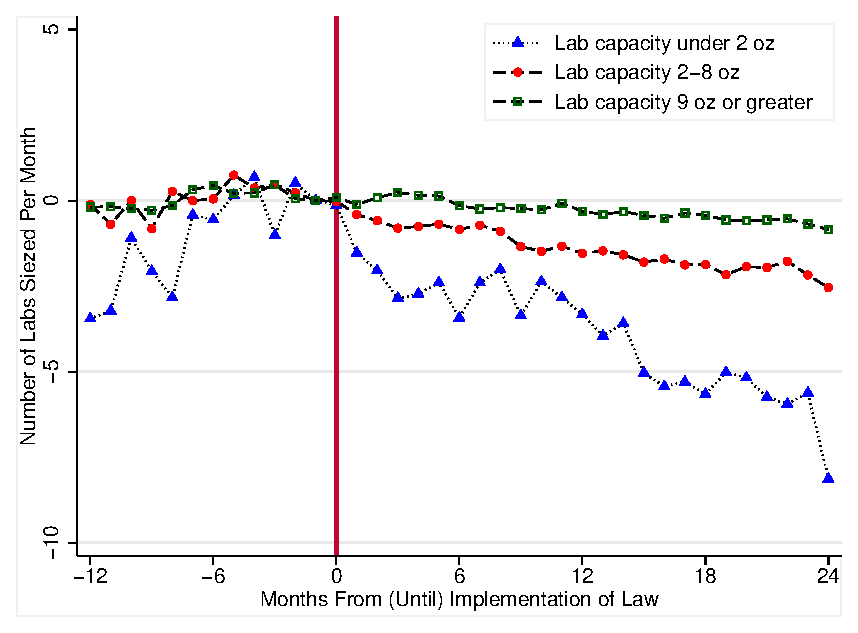
\includegraphics{event-study.eps}
 \caption{Methamphetamine labs discovered or seized by capacity, event study.}
\label{event-study}
\end{figure}

\begin{figure}[!hbtp]
 \centering
 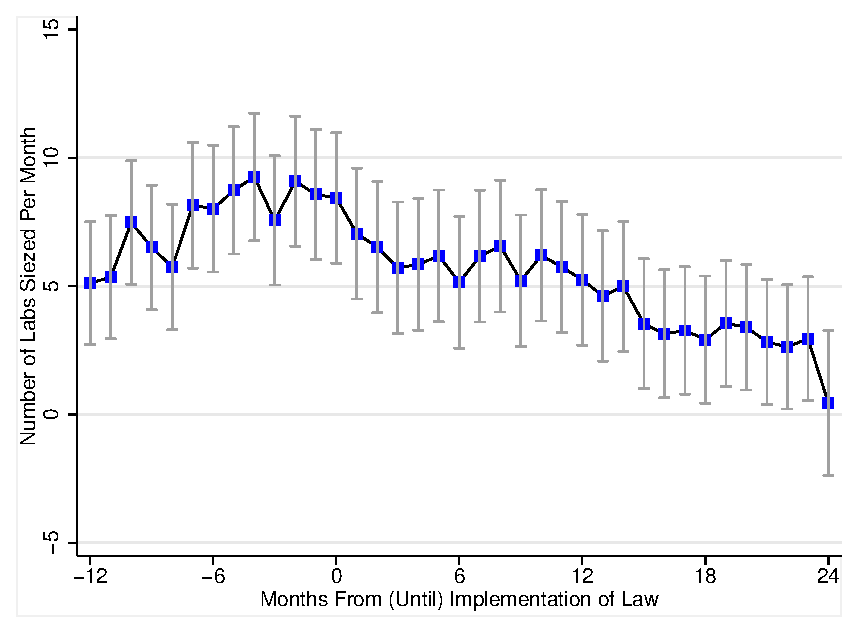
\includegraphics{confidence-interval-plot-for-cap_under_2_oz.eps}
 \caption{Event Study: Methamphetamine Labs Discovered or Seized With Capacity Under 2 oz}
\label{ci-cap2}
\end{figure}

\begin{figure}[!hbtp]
 \centering
 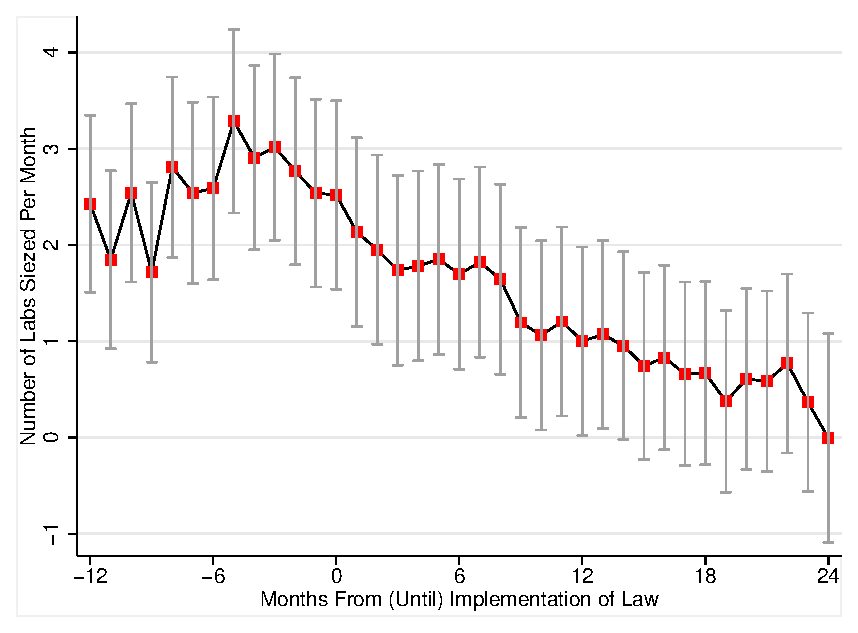
\includegraphics{confidence-interval-plot-for-cap_2_8_oz.eps}
 \caption{Event Study: Methamphetamine Labs Discovered or Seized With Capacity Between 2 and 8 oz}
\label{ci-cap2-8}
\end{figure}

\begin{figure}[!hbtp]
 \centering
 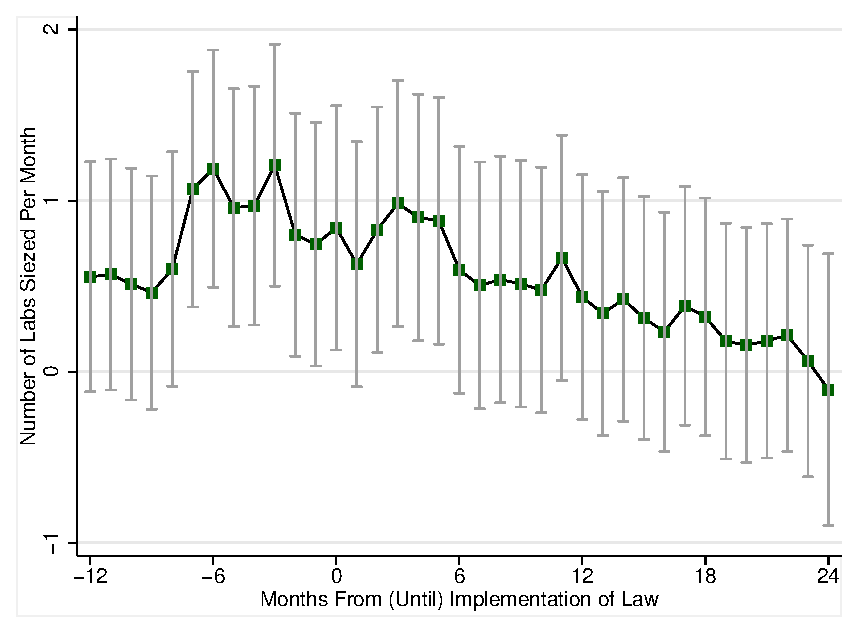
\includegraphics{confidence-interval-plot-for-cap_above_9_oz.eps}
 \caption{Event Study: Methamphetamine Labs Discovered or Seized With Capacity Greater than 9 oz}
\label{ci-cap9}
\end{figure}

\newpage

\hypertarget{references}{%
\section*{References}\label{references}}
\addcontentsline{toc}{section}{References}

\hypertarget{refs}{}
\begin{cslreferences}
\leavevmode\hypertarget{ref-Abadie2017}{}%
Abadie, Alberto, Susan Athey, Guido W Imbens, and Jeffrey Wooldridge.
2017. ``When Should You Adjust Standard Errors for Clustering?'' Working
Paper 24003. Working Paper Series. National Bureau of Economic Research.
\url{https://doi.org/10.3386/w24003}.

\leavevmode\hypertarget{ref-DOBKIN201448}{}%
Dobkin, Carlos, Nancy Nicosia, and Matthew Weinberg. 2014. ``Are
Supply-Side Drug Control Efforts Effective? Evaluating Otc Regulations
Targeting Methamphetamine Precursors.'' \emph{Journal of Public
Economics} 120: 48--61.
\url{https://doi.org/https://doi.org/10.1016/j.jpubeco.2014.07.011}.
\end{cslreferences}

\end{document}
